\documentclass{report}

\usepackage{mathtools}
\usepackage{amsmath}
\usepackage{amsfonts}
\usepackage{amsthm}
\usepackage{amssymb}

\theoremstyle{plain}
\newtheorem{thm}{Theorem}
\newtheorem{lem}[thm]{Lemma}
\newtheorem{prop}[thm]{Proposition}
\newtheorem*{cor}{Corollary}

\theoremstyle{definition}
\newtheorem{defn}{Definition}
\newtheorem{conj}{Conjecture}
\newtheorem{exmp}{Example}

\theoremstyle{remark}
\newtheorem*{rem}{Remark}

\usepackage{tikz}
\usetikzlibrary{arrows,decorations.markings}
\usetikzlibrary{cd}


\usepackage{etoolbox}
\listadd{\pc}{$C$}
\listadd{\pc}{$C\sharp$}
\listadd{\pc}{$D$}
\listadd{\pc}{$E\flat$}
\listadd{\pc}{$E$}
\listadd{\pc}{$F$}
\listadd{\pc}{$F\sharp$}
\listadd{\pc}{$G$}
\listadd{\pc}{$G\sharp$}
\listadd{\pc}{$A$}
\listadd{\pc}{$B\flat$}
\listadd{\pc}{$B$}
\usepackage{calc}



\usepackage[top=2.5cm, left=3cm, right=3cm, bottom=2.5cm]{geometry}
\usepackage{caption}
\captionsetup{margin=10pt,font=small,labelfont=bf}


\begin{document}



%\begingroup
\title{Categories and music}
\author{Alice Rixte}
\date{\today}
\maketitle %\endgroup


\chapter{Introduction}


\section{Presentation of Allen Forte's work}
\begin{defn}
    A \textbf{pitch class} consists of all the pitches separated with a whole number of octaves.
\end{defn}
The set of all pitch classes comes naturally with a group structure, which is actually the group $\mathbb{Z}_{12}$. Indeed, we can associate $C$ to the pitch class $0$, $C\sharp$ to the pitch class $1$ and so on. We then have the possibillity to represent a $C$ major chord  from a geometrical point of vue (see Figure \ref{Cmajor}).

\newcounter{itemcount}
\setcounter{itemcount}{450}
\renewcommand*{\do}[1]{
    \filldraw [black]  (\number\value{itemcount}:3cm) circle (1.5pt)
    node[anchor={\number\value{itemcount}-180}]
        {#1\addtocounter{itemcount}{-30}};
}

\begin{figure}[ht]
    \centering
    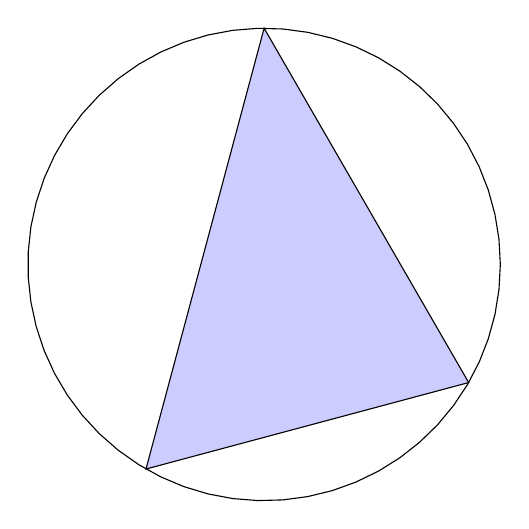
\begin{tikzpicture}
        \dolistloop{\pc}
        \draw[fill=blue!20] (90:3cm) -- (330:3cm) -- (240:3cm) -- cycle;
        \draw [domain=0:360,samples=60] plot ({3*cos(\x)}, {3*sin(\x)});
    \end{tikzpicture}
    \caption{The C Major chord in the chromatic circle}
    \label{Cmajor}
\end{figure}

The idea of Forte relies on the fact that a major chord will always have the same representation up to 12 rotations in this geometrical paradigm. In mathematics they are the 12 rotational symmetries of the regular dodecahedron.In music theory, these rotations are called \textbf{transpositions} and are named $T_i$ for $i\in[\![0,11]\!]$.

His intuition was that instead of considering triads (three notes chord) as the set of the notes that compose them, we should consider them as the set of the intervals between each note. As a result, every inversion of chord \footnote{the term inversion has to be taken here from a musical point of view, for instance the inversions of a C major chord are C-E-G, G-C-E, E-G-C. Later in this report, we will use inversion with another definition and we will stick to it.} will be in the same \textbf{pitch-class set}\cite{forte_1980}. This can be seen in the geometrical point of view where the simple fact  of representing the chord as a triangle allow to forget any order between the three note. Similarly, all the transpositions of the chord will be in the same pitch-class.

\paragraph{Contribution (sort of)}
From another point of view, the work of Forte can be seen as networks, as in Figure \ref{transpose_net}. Nonetheless, this representation does not allow for the moment to embed the notion of pitch-class set of Forte. For this we have to introduce the Klumpenhouwer networks.
\begin{figure}[ht]
    \centering
    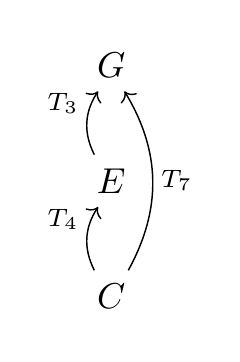
\begin{tikzpicture}[baseline= (a).base]
        \node[scale=1.3] (a) at (0,0){
            \begin{tikzcd}
                G                                                            \\
                E \arrow[u, "T_3", bend left]                                \\
                C \arrow[u, "T_4", bend left] \arrow[uu, "T_7"', bend right]
            \end{tikzcd}};
    \end{tikzpicture}
    \caption{Transpositional network}
    \label{transpose_net}
\end{figure}

\section{Presentation of Klumpenhouwer networks}
In  the 1980s, David Lewin developped a branch of music theory called transformational theory\cite{rahn_lewin_1987}. It consists of, rather than looking the musical objects for themselves but instead to mathematically study the relation between them.
%TODO read rahn_lewin_1987

Klumpenhouwer networks, or K-nets, were then introduced by Henry Klumpenhouwer, former PhD student of Lewin, to formalize the relation between two chords\cite{lewin_1990}.

We have seen that the rotations of the dodecahedron match with the notion of transposition. However, there another type of symmetry in the dodecahedron : the $12$ reflexion symmetries (see Figure \ref{inversions}), called \textbf{inversions} in transformational music theory. Along with transposition, they form the $T/I$ group, otherwise known in mathematics as the \textbf{dihedral group} of a dodecahedron.

\setcounter{itemcount}{450}

\begin{figure}[ht]
    \centering
    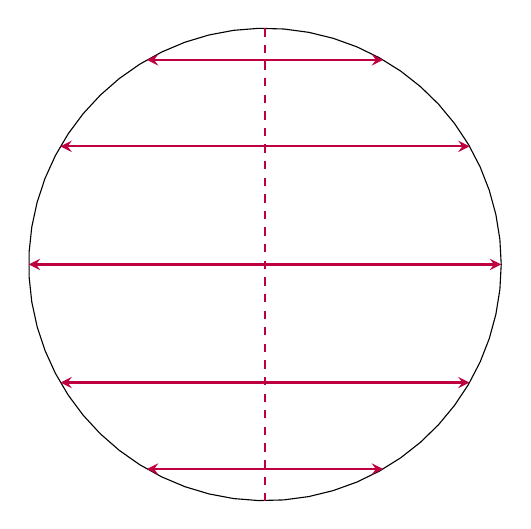
\begin{tikzpicture}
        \tikzset{myptr/.style={decoration={markings,mark=at position 1 with %
                                {\arrow[scale=3,>=stealth]{>}}},postaction={decorate}}}
        \dolistloop{\pc}
        \draw [domain=0:360,samples=60] plot ({3*cos(\x)}, {3*sin(\x)});
        \draw [dashed,purple] (90:3cm) -- (270:3cm);
        \foreach \i in {1,...,5}{
                \draw [<->, >=stealth, thick, purple] (90 + \i*30:3cm) -- (90-\i*30:3cm) ;
            }

    \end{tikzpicture}
    \caption{The $I_0$ inversion}
    \label{inversions}
\end{figure}

The idea behind K-nets is that instead of analyse chords transformations threw transposition only, which is not very rich, we could instead use also inversions.

\begin{defn}
 A Klumpenhouwer network is a network where objects are pitch classes and arrows between objects are labeled by an element of the 
\end{defn}


\section{Presentation of PK-nets}

PK-nets\cite{PAAE2016} are the generalization of the


\begin{defn}\textbf{Set} is the category where objects are the sets and morphisms are functions between sets.\end{defn}


\begin{figure}[ht]
    \centering
    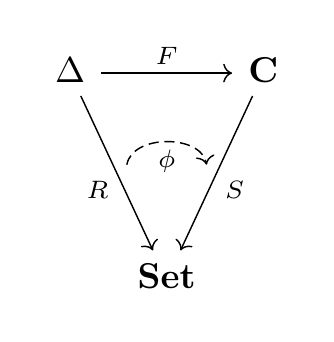
\begin{tikzpicture}[baseline= (a).base]
        \node[scale=1.3] (a) at (0,0){
            \begin{tikzcd}[column sep=tiny]
                \Delta \ar[ddr, "R"',""{name=R,right}] \ar[rr,"F"]	& & \textbf{C} \ar[ddl,"S",""{name=S,left}] \\
                & \ar[dashed,bend left=80,from=R, to=S, "\phi"']& \\
                & \bf Set &
            \end{tikzcd}
        };
    \end{tikzpicture}
    \caption{PK-net definition}
\end{figure}





\subsection{Recover Tonnetz}


\begin{defn} The \textbf{category of elements} $el(F)$ of a functor $F : \mathcal{C}\rightarrow \textbf{Set}$ is defined as follows :
    \begin{itemize}
        \item its objects are the pairs $(c,x)$ where $c$ is an object of $\mathcal{C}$ and $x\in F(c)$
        \item its morphisms $(c,x)\rightarrow (c',x')$ are morphisms $u : c\rightarrow c'$ such that $F(u)(x) = x'$
    \end{itemize}
\end{defn}
\paragraph{}
Now, what is the category of elements of the PLR-group action over \textbf{Set}? Let $S$ be the functor from the category PLR to the category \textbf{Set} such that $S$ associates to the only object of PLR a set $X$ of cardinality 24 and such that $S$ is a PLR-group action on $X$.

$el(S)$ is then a category with $24$ objects. One can use it as a $\Delta$ category in a PK-net. The transformation $\phi$ gives us the musical interpretation, of each transformation triads.

=> How to add more structure to eliminate arrow? Maybe take two generators



\begin{defn}
    The \textbf{free strict monoidal category} $ \Sigma (C)$ over a category $C$ is a monoidal category such that :
    \begin{itemize}
        \item objects of $\Sigma (C)$ are the list of objects of $C$
        \item for two objects $A = A_1,\dots,A_m$ and $B = B_1,\dots,B_n$ of $\Sigma (C)$, if $m = n$ then every list of morphisms $f_1,\dots,f_m$ such that $f_i$ is a morphism from $A_i$ to $B_i$ in $C$ is a morphism of $\Sigma(C)$ from $A$ to $B$
        \item The tensor product of two $\Sigma(C)$ objects is there concatenation as well as the tensor product of two morphisms.
    \end{itemize}
\end{defn}


\paragraph{Strict monoidal category freely generated by a group}



Let $G$ be a group seen as a one-element category. Then $ \Sigma(G)$ is a category such that : 
\begin{itemize}
    \item $\Sigma(G)$ has a countable infinity objects : the lists $A_n$ of length $n \in \mathbb{N}$ and where all the elements of $A_n$ are $A$.
    \item Since there is only one object of length $n$, there is no morphism between two different objects of $\Sigma(G)$. Let's consider the full subcategory containing only the $A_n$ object. Then the morphisms of this category are of the form $f_1,...,f_n$ where $f_i$ is a morphism from $G$. We recognize the group $G^{n}$. $\Sigma (G)$ is then the disjoint union of the $G^{n}$ for $ n\in\mathbb{N}$.
    \item  The tensor product is such that  $A_m \otimes A_n = A_{m+n}$, or, in other words, $G^m \otimes G^n = G^{m+n}$. 
\end{itemize}



\chapter{Conclusion}

\newpage

\bibliography{bibliography}
\bibliographystyle{ieeetr}
\end{document}